\documentclass[10pt,a4paper]{article}
\usepackage[utf8]{inputenc}
\usepackage{amsmath}
\usepackage{amsfonts}
\usepackage{amssymb}
\usepackage{graphicx}
\usepackage{enumerate}
\begin{document}

\section{Set Theory}

To demystify mathematics consider
\begin{enumerate}[(i)]
\item What is a theorem?
\item What is a proof?
\end{enumerate}
What if we don't know the answer?

To begin we need
\begin{enumerate}[(a)]
\item an example(s)
\item a nearly related concept
\end{enumerate}


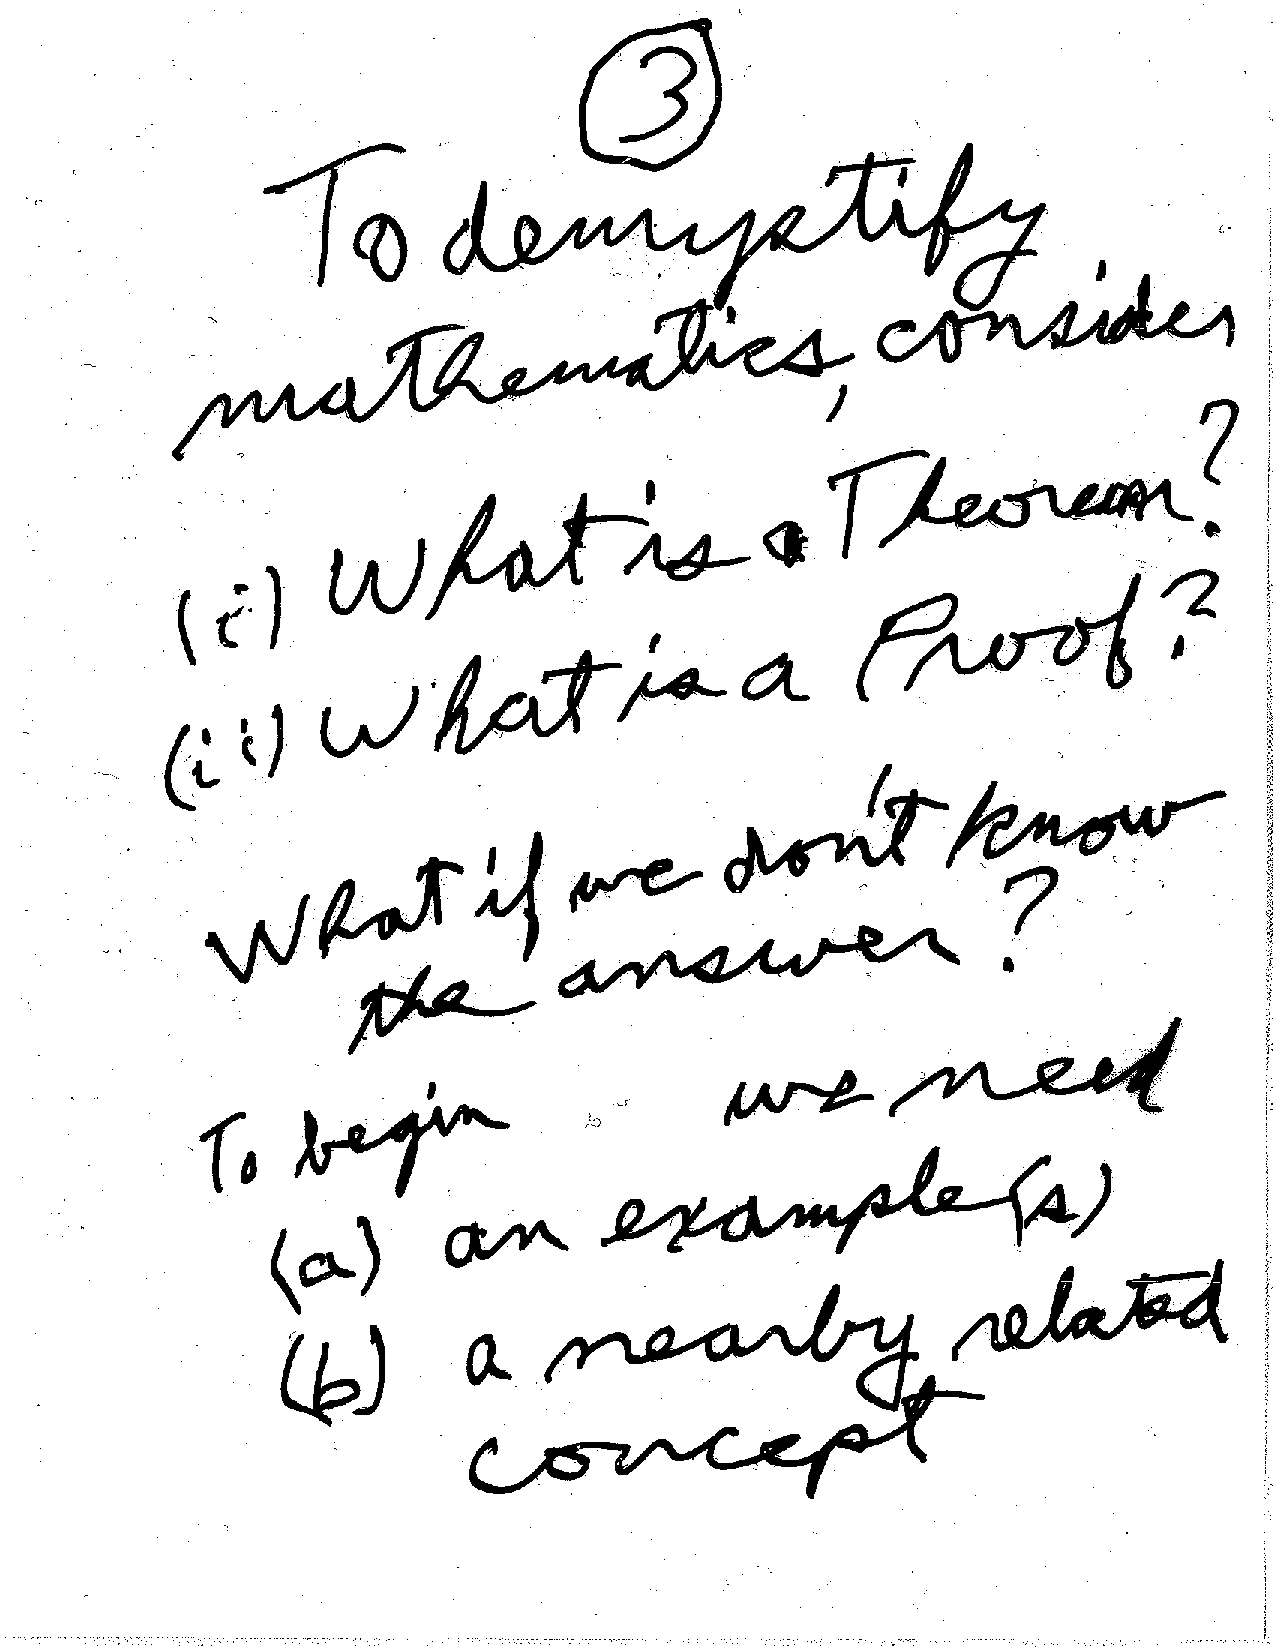
\includegraphics[scale=.5]{Pages/ST_3}

\newpage

Related Concept: Greek Syllogism

\underline{example:}
\begin{enumerate}
\item All men are mortal.
\item Socrates is a man.
\item Therefore, Socrates must die. 
\end{enumerate}

To analyze, recast in set theoretic terms via Venn Diagram.

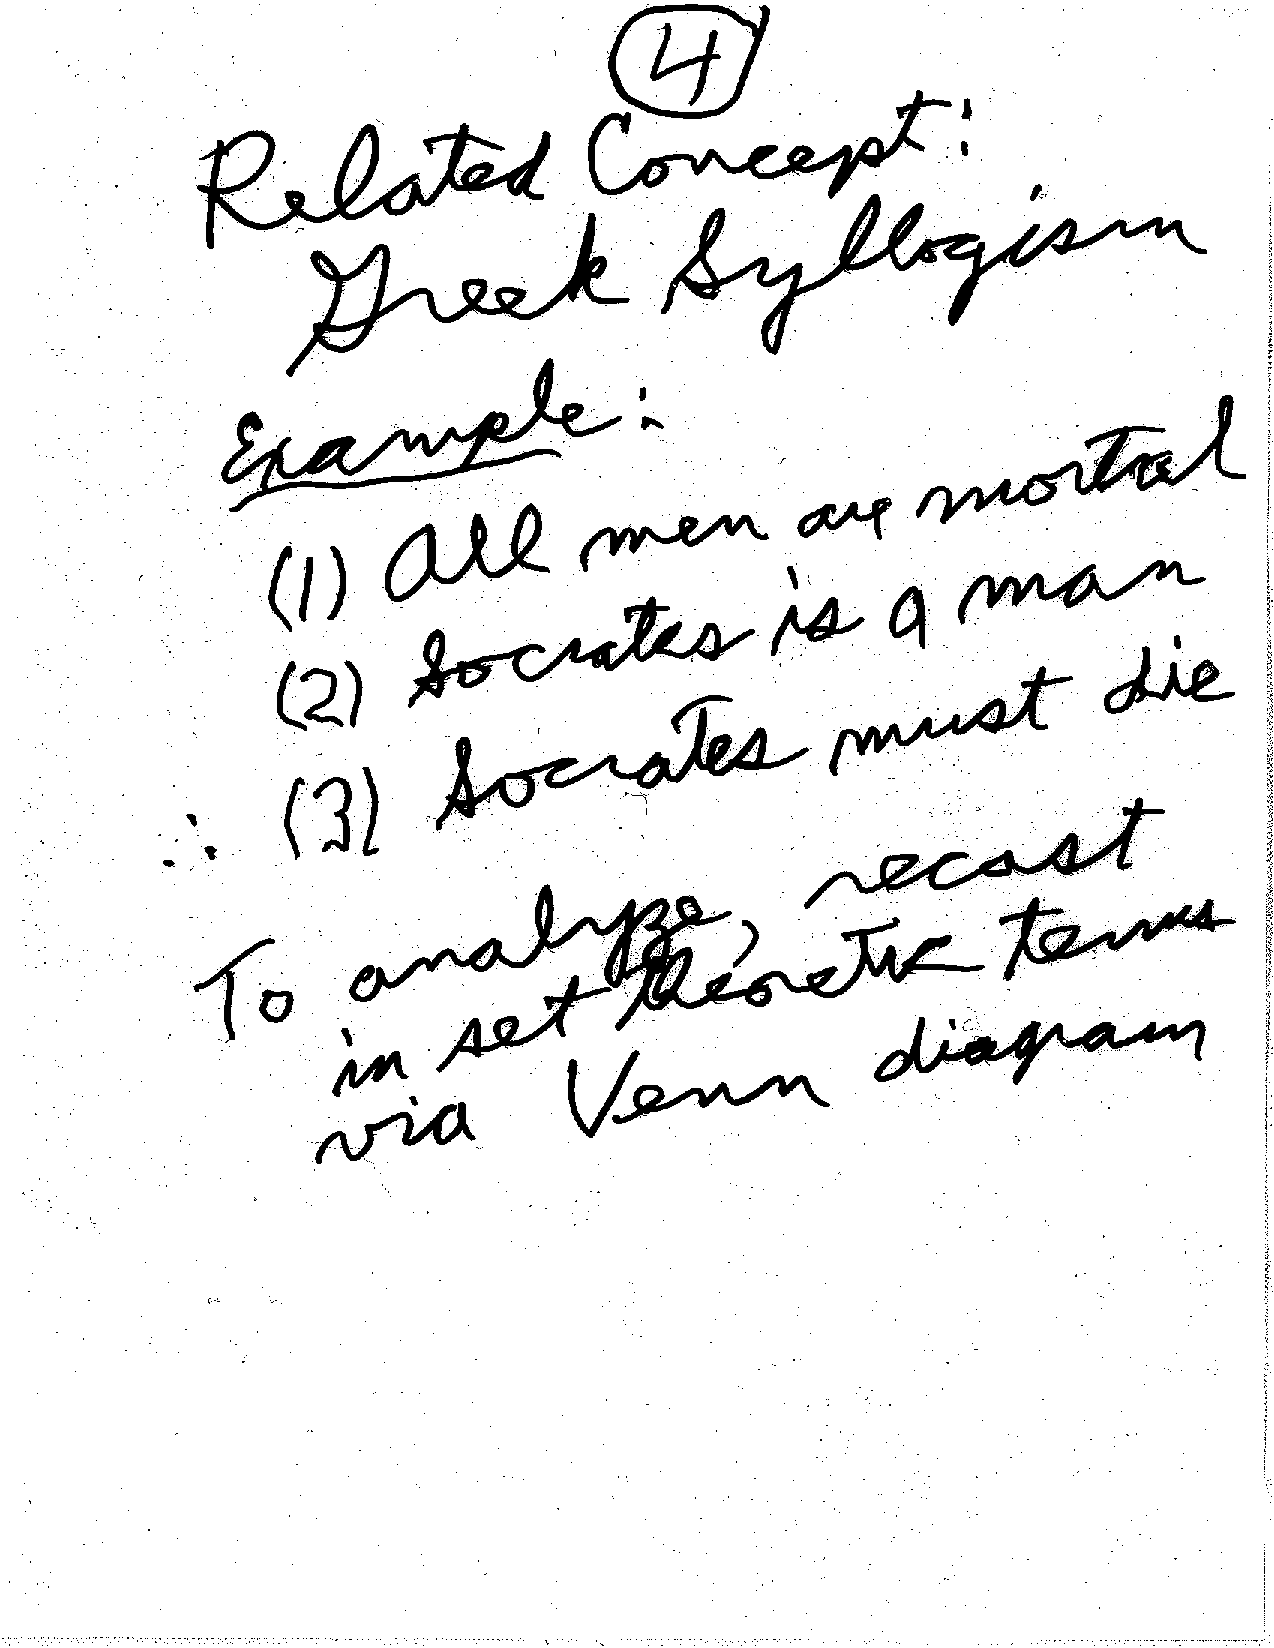
\includegraphics[scale=.5]{Pages/ST_4}

\newpage

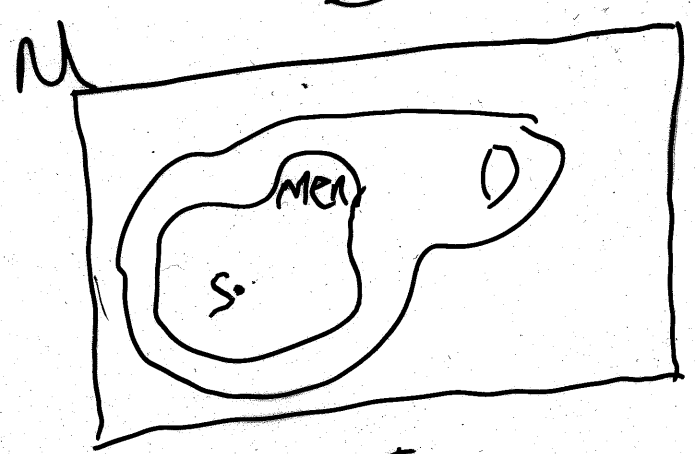
\includegraphics[scale=.2]{Pages/ST_5_im1}

$S$: Socrates\\
$M$: Set of Men\\
$D$: Things that will die\\
$\mathcal{U}$: Things on Earth

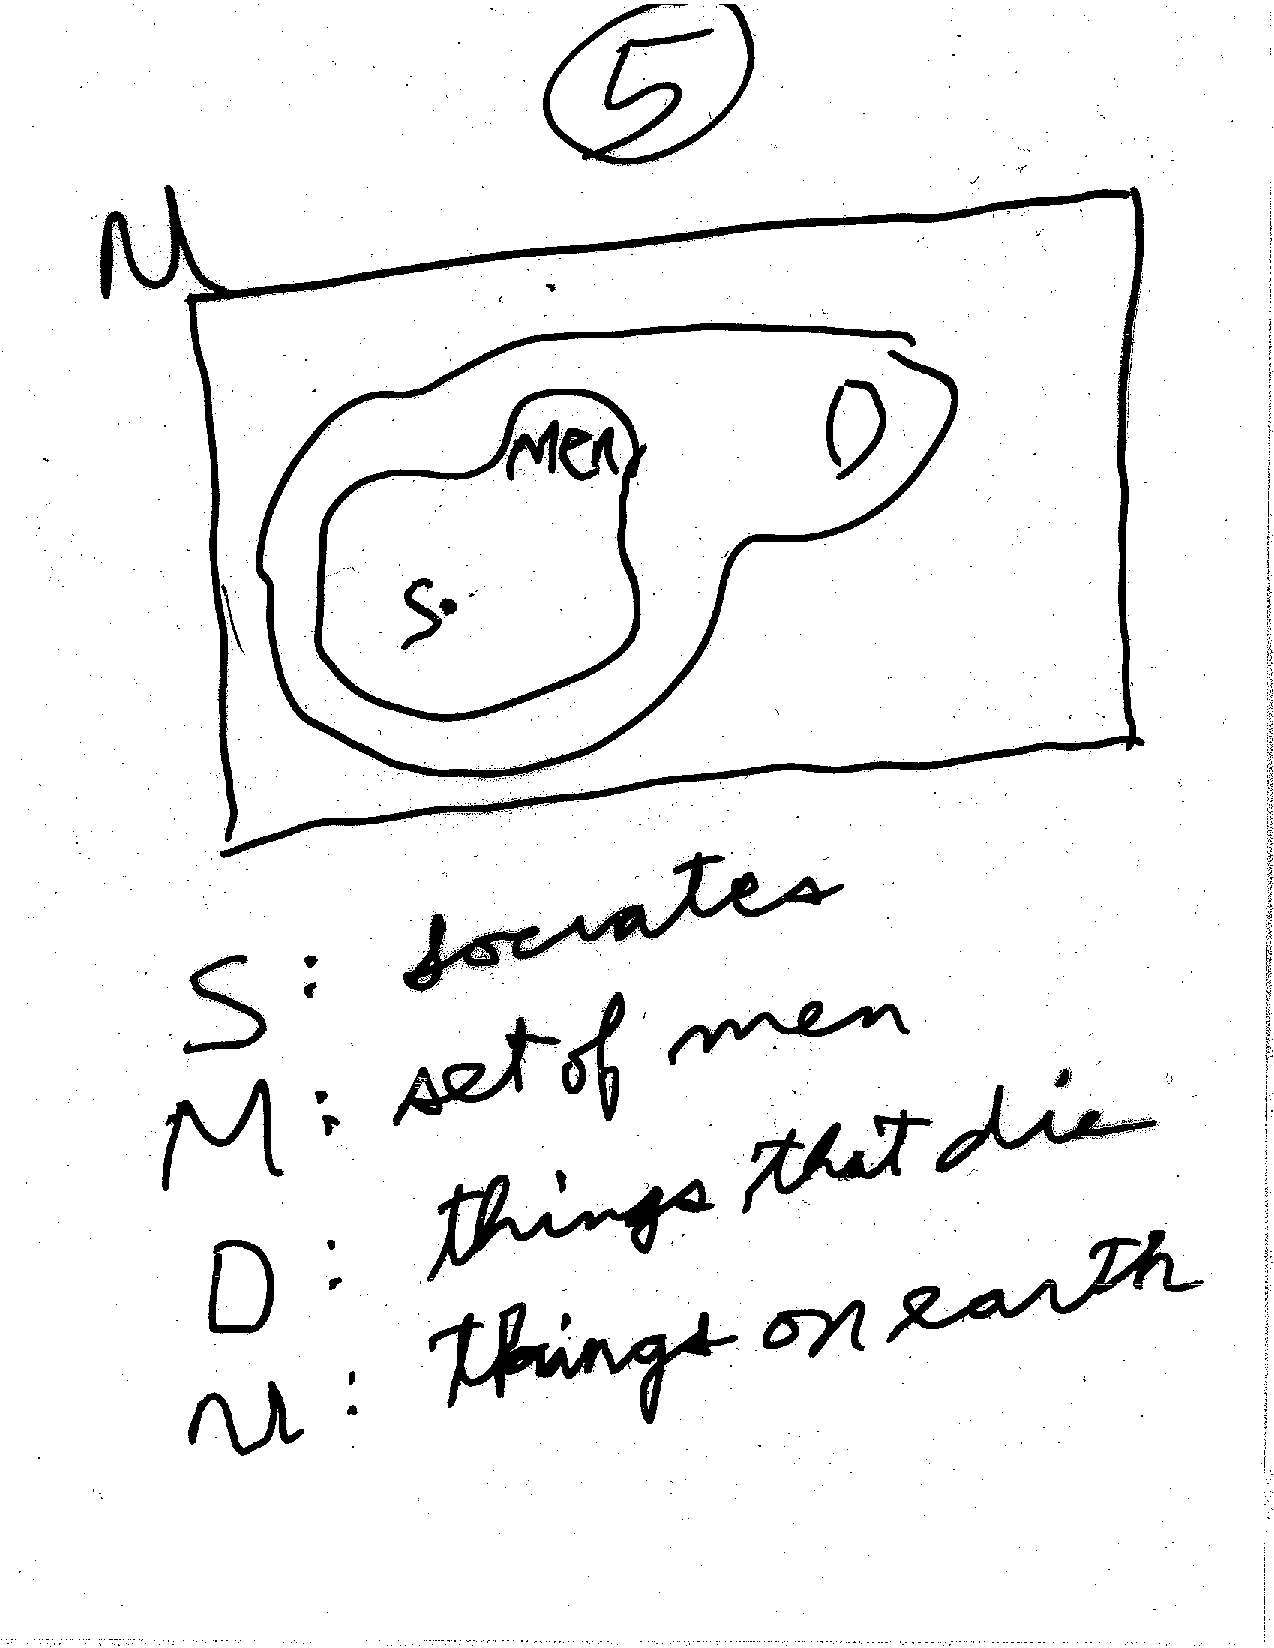
\includegraphics[scale=.5]{Pages/ST_5} 



%Zack: Pages 6,7,8,19,20

%Jack: 21, 9, 10, 11

%Koka: Pages 13, 13A, 22 ,22A, 22B


\section{Generate $\mathbb{N}$}


%Ruth: Pages L4A-L4G




\section{From $\mathbb{Z}$ to $\mathbb{R}$ via ordering}
%Jazz: ZR1-ZR5

%Kyler: ZR6 - ZR10

%Preethika: ZR11-ZR14


\section{Sequence and Limits}

%Aaron: First 2 pages and 48-50

%Hamza: 51-52B

\section{Limit and Convergence}

%Joe: 50-51

%Quinten: 52-53
Therm Let $\{ a_n \}$ be monotonic
in $\mathbb{R}$. Then in $\mathbb{R}_{\infty}$
$\lim_{n \rightarrow{\infty}}$
$$a_n = \begin{cases} 
\sup \{ a_k \} & \mbox{if } a \leq a_2 \leq a_3 \leq...\\
\inf \{ a_k \} & \mbox{if } a\geq a_2 \geq...
\end{cases}$$

The limit is in  $\mathbb{R}$ if $\{ a_n \}$ is bounded


$\underline{Pf}$: WL.o.g spse  $a_1 \leq a_2 \leq ...$ Take any b $<$ sup $\{ a_k \}$ Then 

$\exists\ k_* < \infty$ s.t. $b < a{_k{_*}}$ for all $n \geq k_* , \{ a_n \} \geq 
 a{_k{_*}}$ so $ a_n > b.$ But also $a_n \leq a_n$
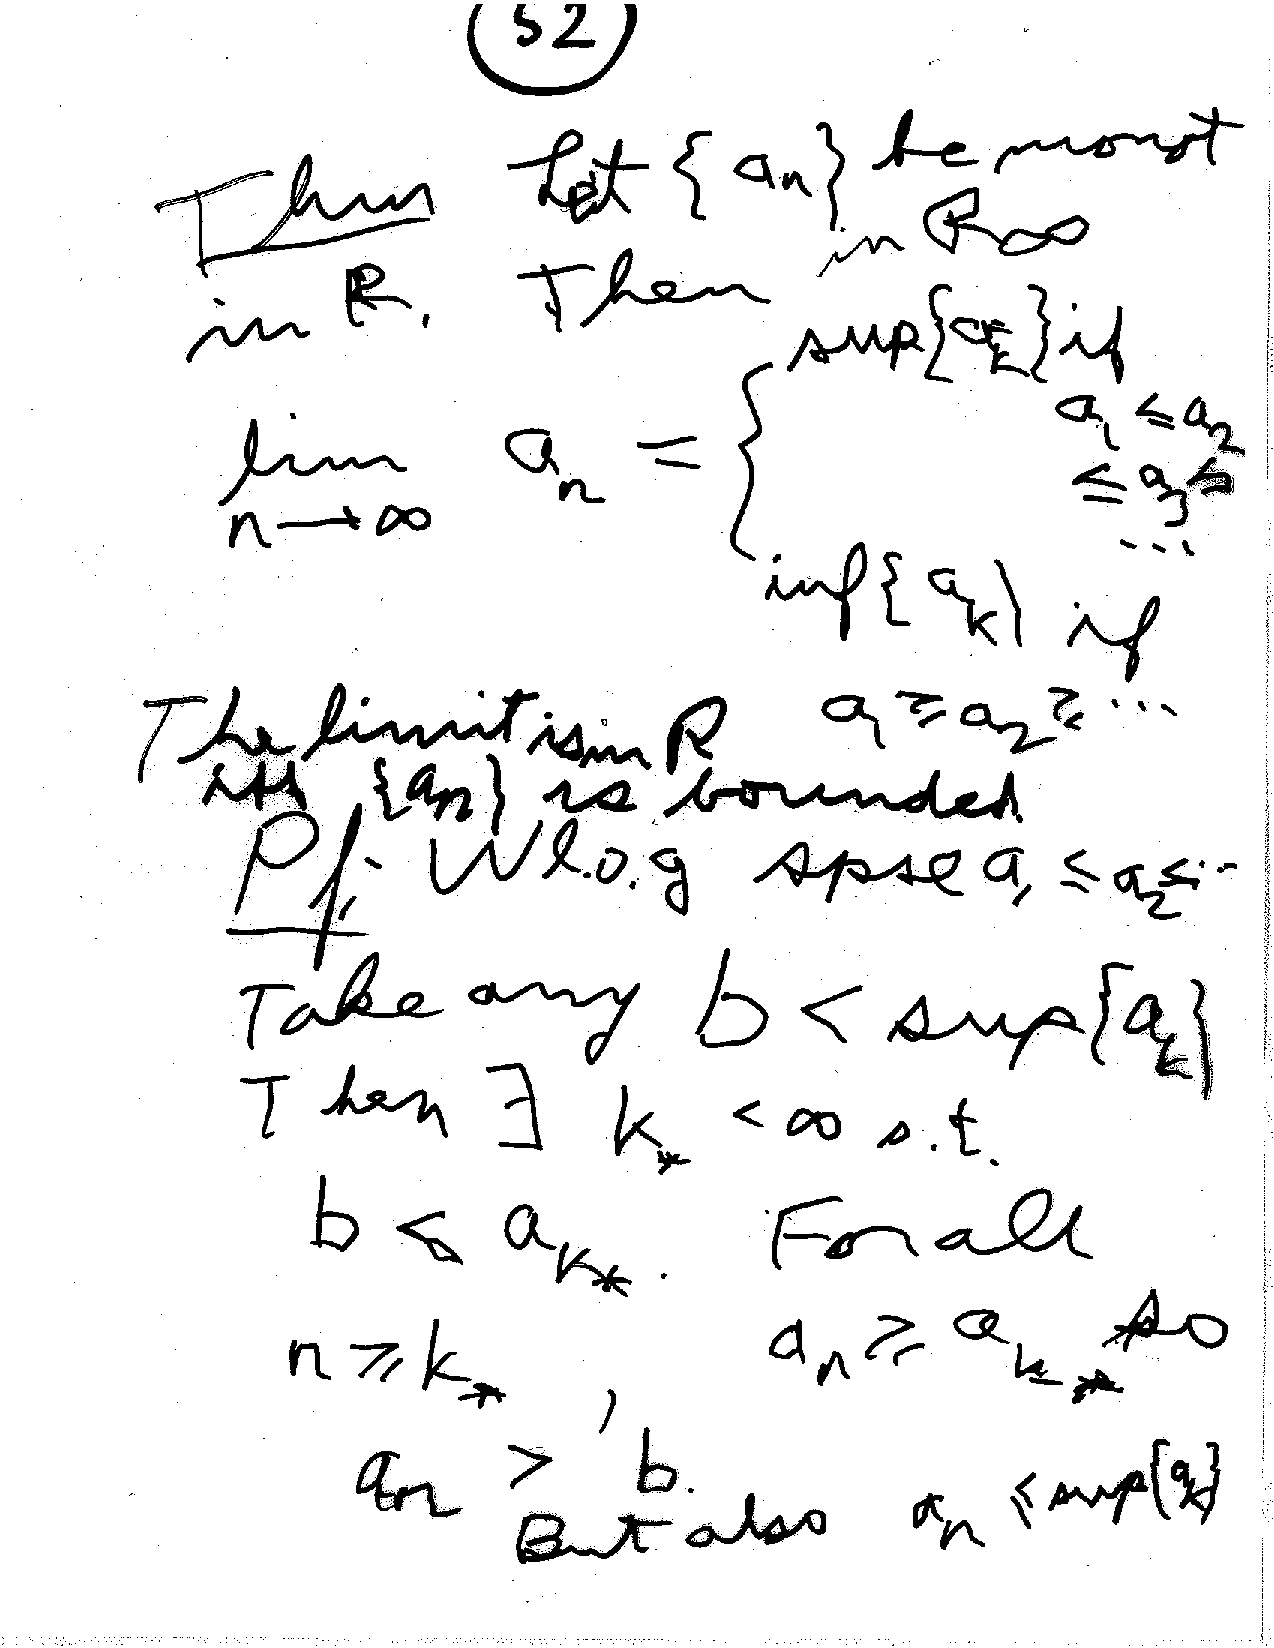
\includegraphics[scale=.5]{Pages/LC_6} 

\newpage
What if $\{ a_n \}$ is $\underline{not}$ monotonic?
$\underline{Therom}$ Let $\{ a_n \}$ be seq in $\mathbb{R}$.
Then $\exists$ 1 $\geq$ n, $<$ $n_2$ $<$ ... s.t. $a_{n_{1}}$,$a_{n_{2}}$, ... is monotonic.
$\underline{Pf}$: We need to consider the tail of a seq. Let 
$$\mbox{J} = \left\{ j \leq | : a_j > a_{j{t{k}}}\ for all\ K \leq 1 \right\}$$

If J is  unbounded we may write $\mbox{J} = \begin{cases} n_j & J\leq 1 \end{cases}$ where $1 \leq n_1 <n_2<...$
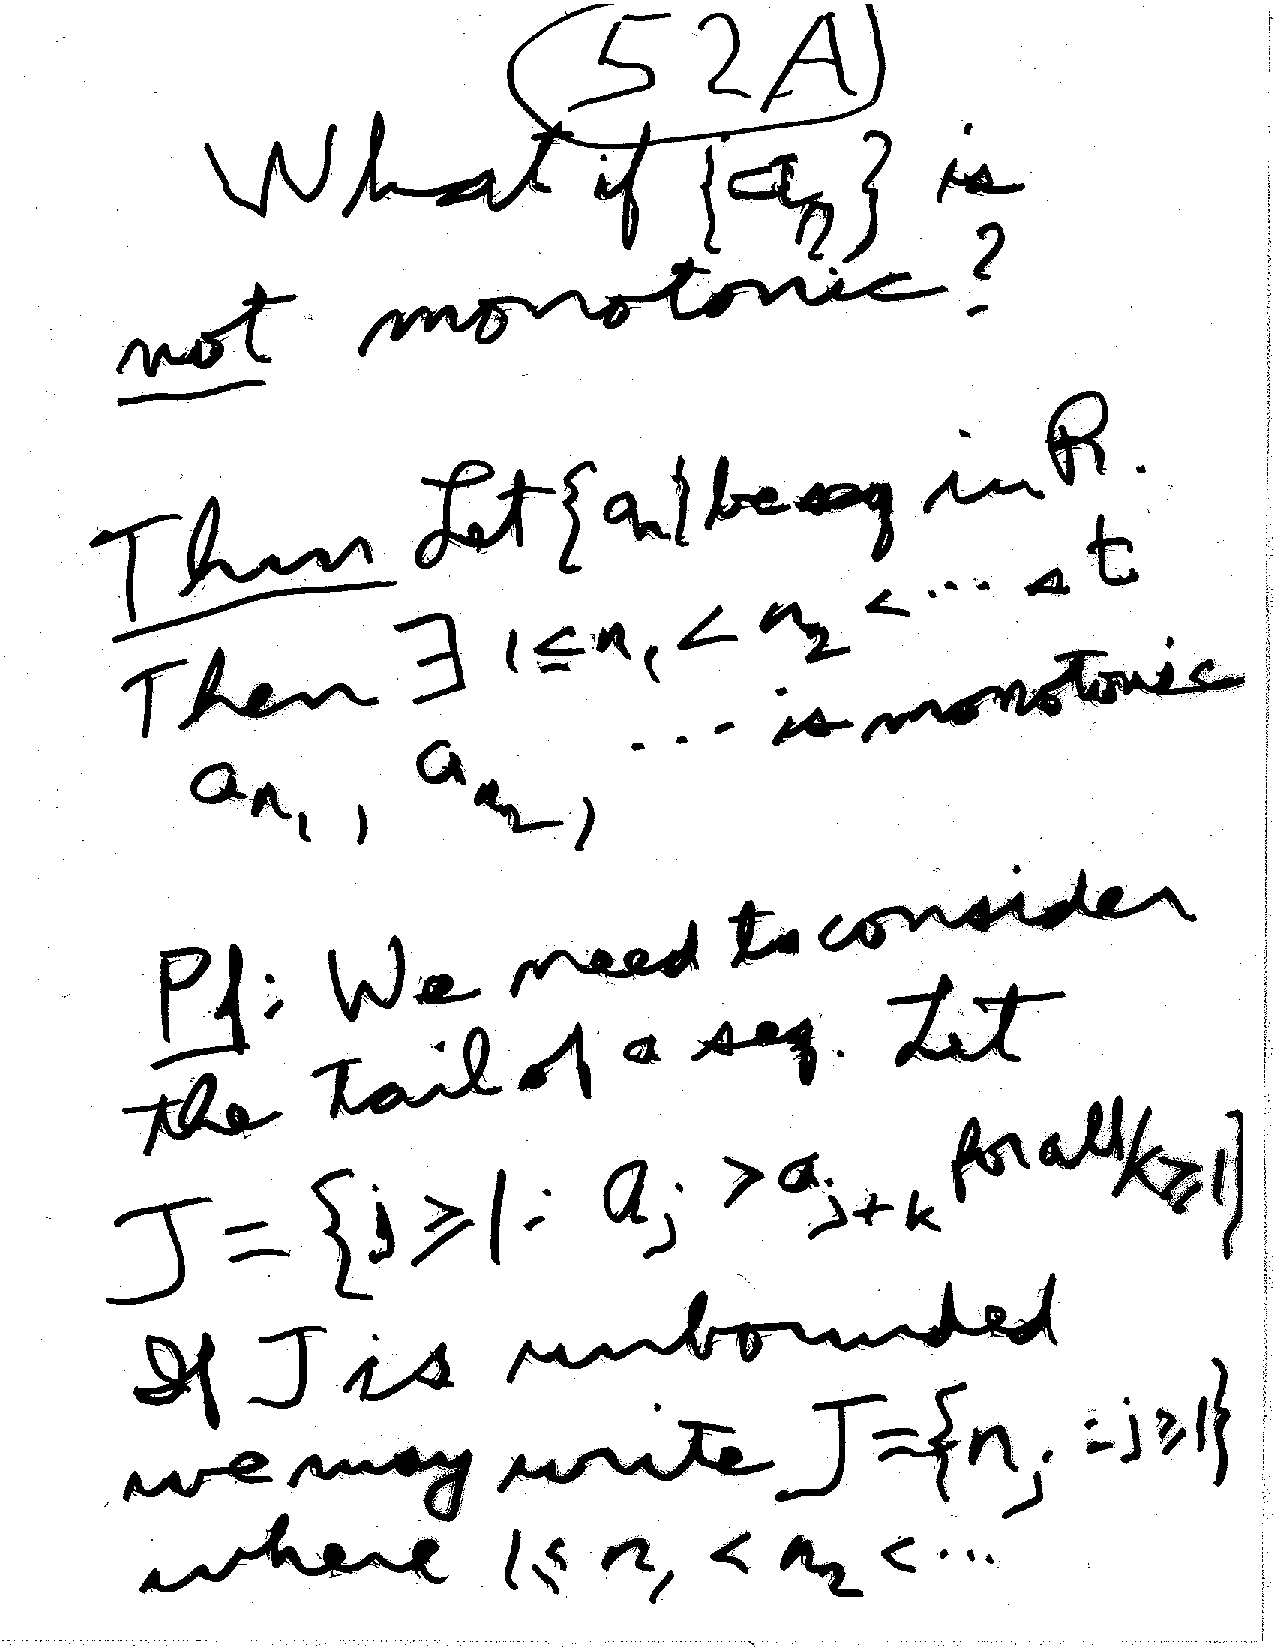
\includegraphics[scale=.5]{Pages/LC_7}

\newpage
By construction, $a_{n_{1}} > a_{n_{2}} >$ ... on the other hand, if $|J| < \infty$, let $n_1 \geq 1$ exceed every j $\in$ J. Having constructed $n_1 < n_2 < ... < n_k$ with $a_{n_{1}} \leq a_{n_{2}} ... \leq a_{n_{K}}$ (since $n_k$ and J) $\exists$ $n_k + 1 > n_k$ s.t. $a_{n_{k}} + 1$, and the desired construction follows by induction.
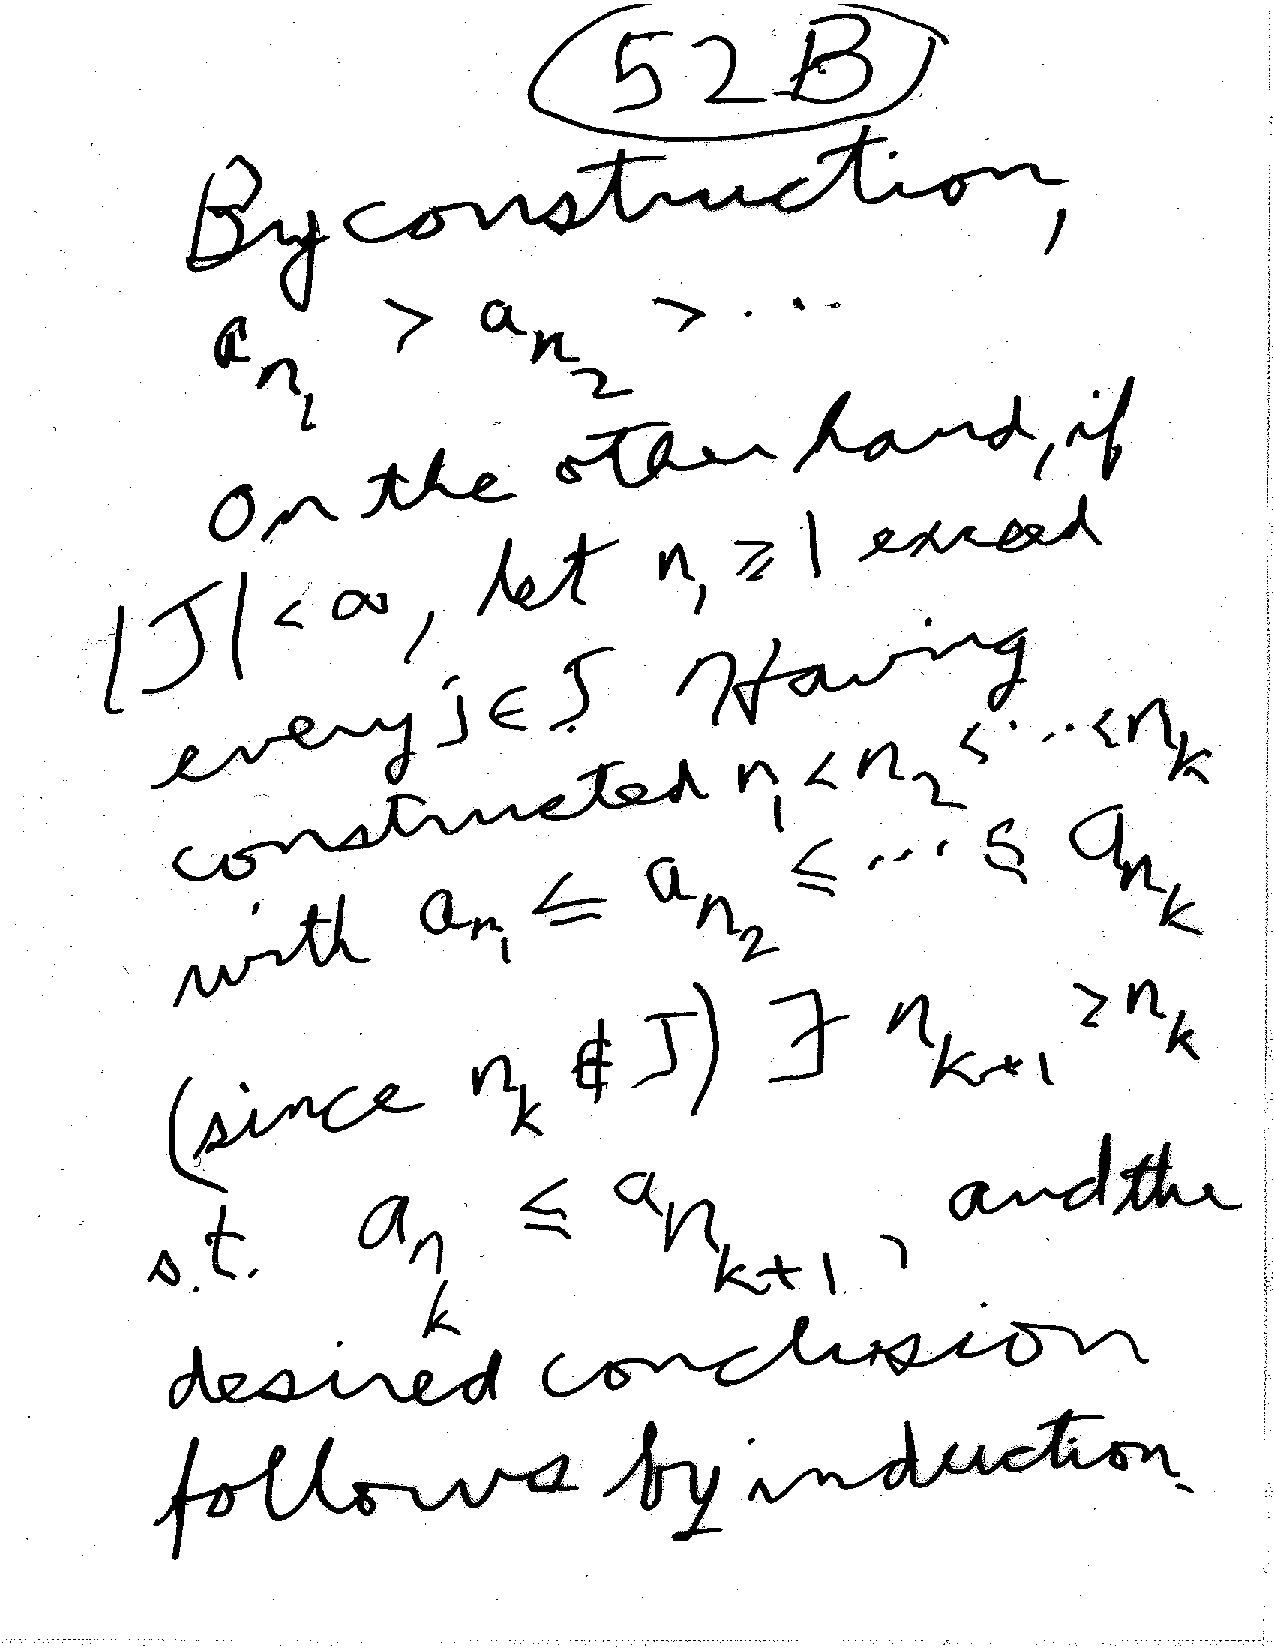
\includegraphics[scale=.5]{Pages/LC_8}

\newpage 
(Balzono weierstras) $\underline{Corllary}$ if $|a_n|$ is a bounded seq in $\mathbb{R}$, it has a covergent subsequence. (Even if $\{ a_n \}$ is $\underline{not}$ bounded, it has a subseq converging in $\mathbb{R}_\infty$.)
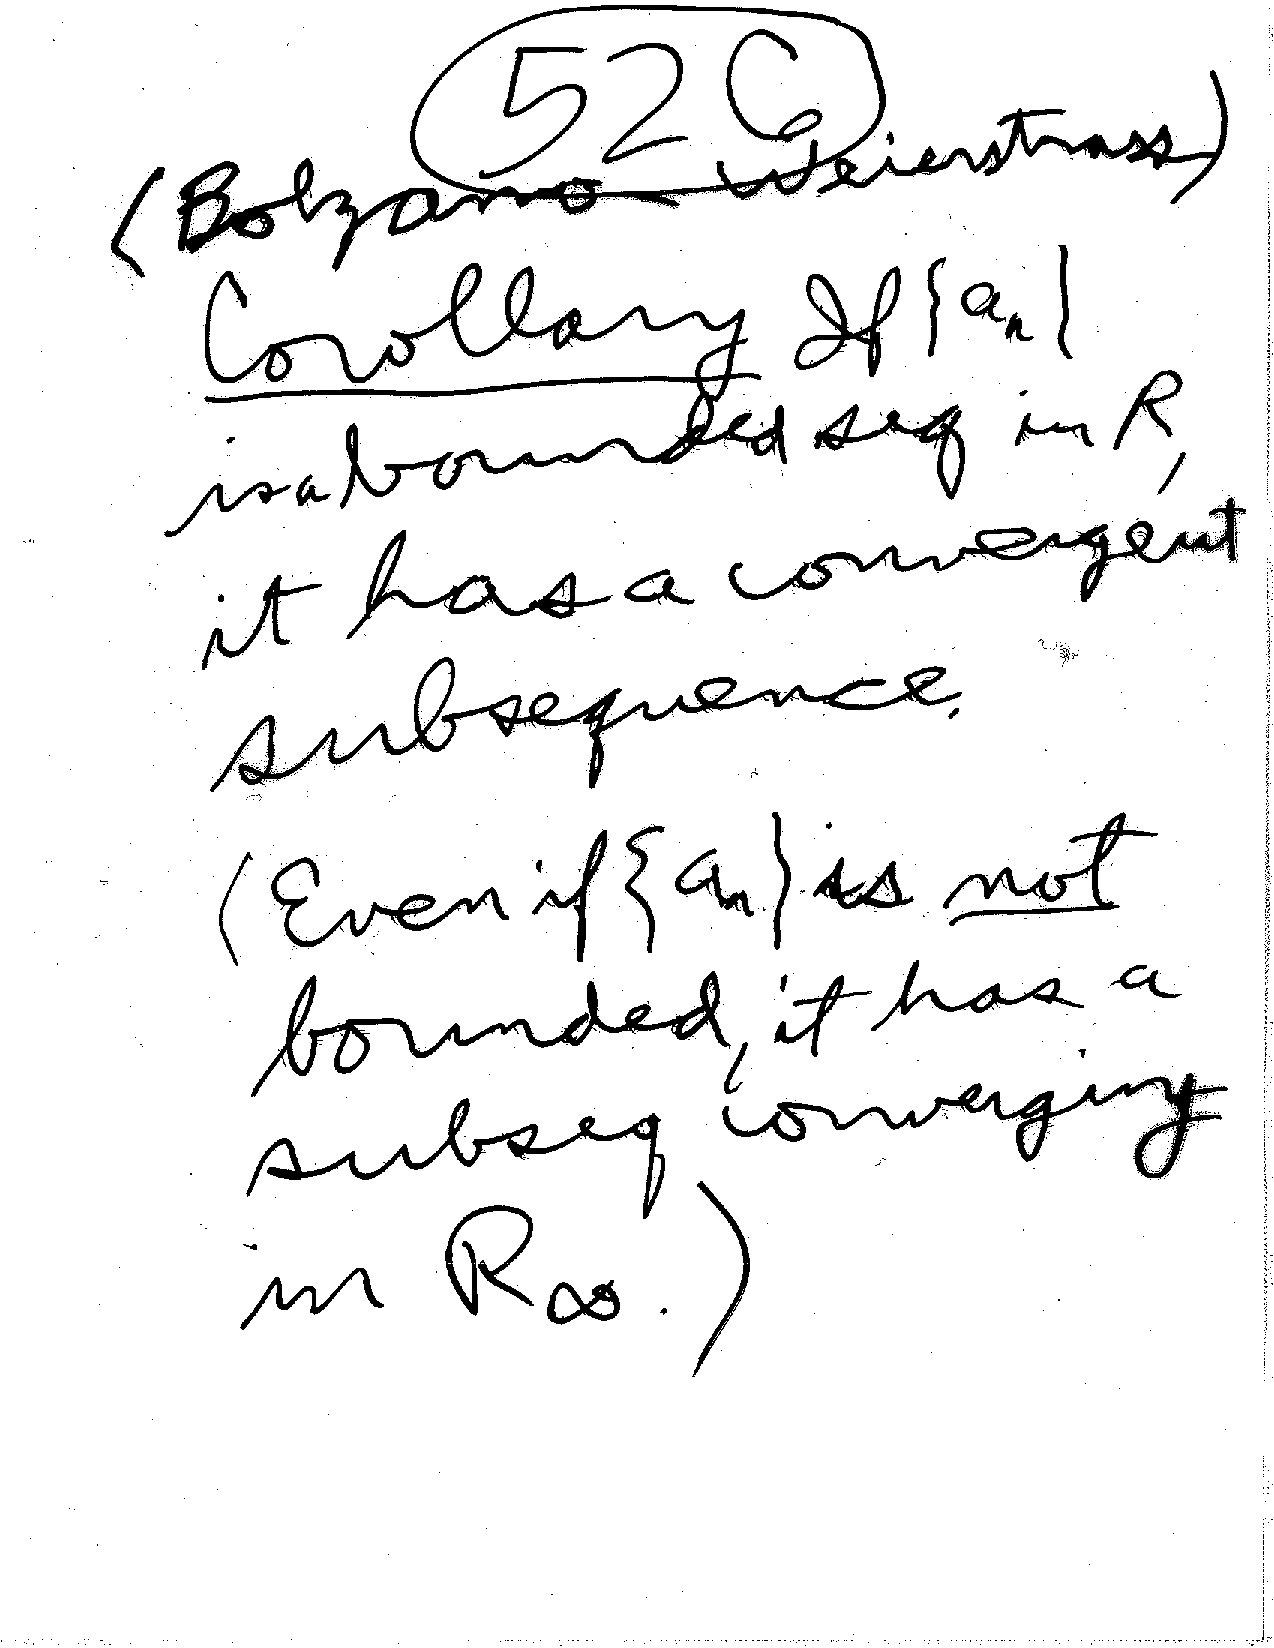
\includegraphics[scale=.5]{Pages/LC_9}

\newpage
$\underline{Cauchy Sequence}$ When can we gaurentee that a seq converges? $\underline{Def}$: a seq of vals $\{ x_n \}$ is said to be a $\underline{Cauchy seq}$ is $\forall \epsilon > 0 \exists N_\epsilon$ such that for every $n,m \geq N_\epsilon$ $$|x_n - x_m| < \epsilon$$ 
$\underline{Prop}$ Spse $x_n \rightarrow x$ Then $\{ x_n \}$ is a Cauchy seq.

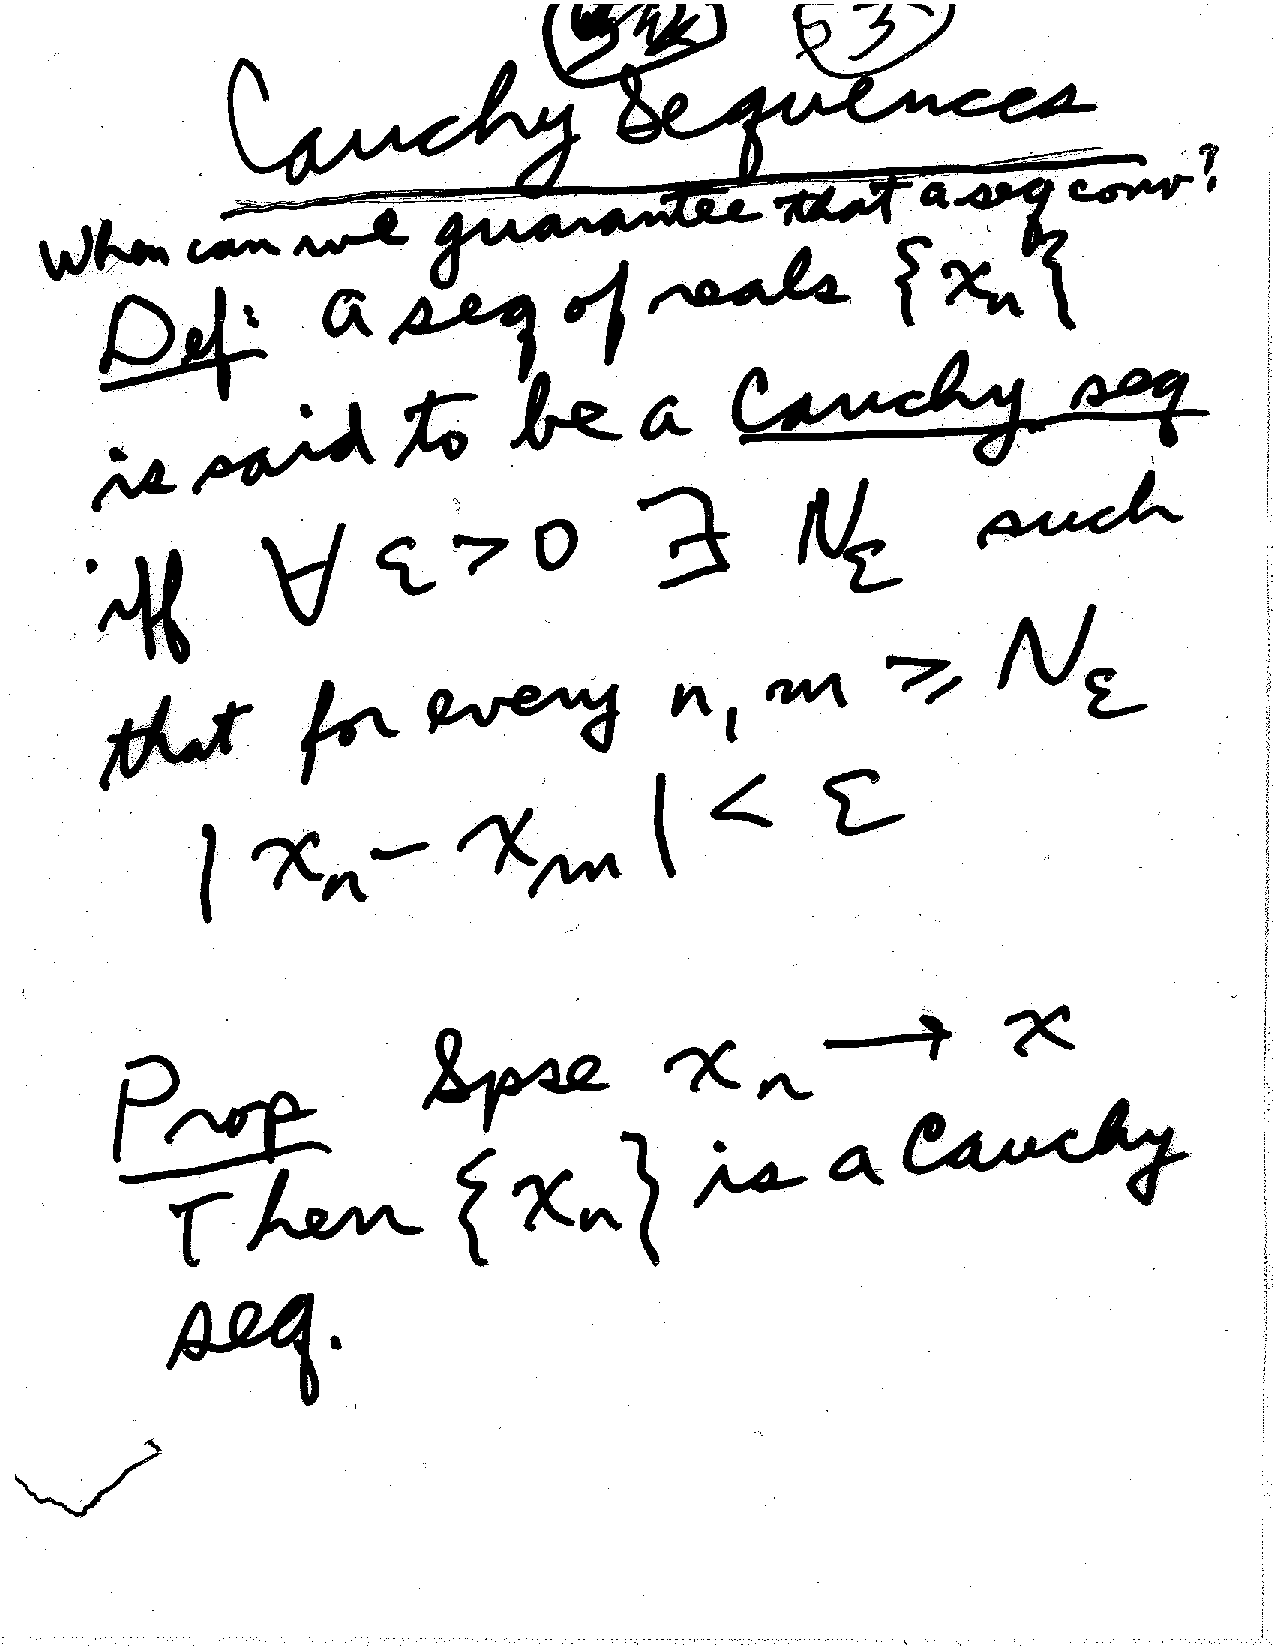
\includegraphics[scale=.5]{Pages/LC_10}

%Farishta: 53A-54A
\newpage
\section{Infinite Series}

%Sukhreet: IS1 - IS 7

%Matthew: IS8 - IS15

%Will: IS16 - IS23

%Rebecca: IS24 - IS32

%Maady: IS33 - IS42

\section{Metric Spaces Part 1}

%Travis: M1 - M5

%Jerome: M6- M10



\section{Metric Spaces Part 2}


%Bryant: M1-M7

%Reshma: M8-M14

%Ethan: M15-M21





\end{document}